\subsection{Comparing with EMV2 Modeling}
\label{subsec:comparison_with_EMV2}
In this section, we use a few examples from the WBS system to illustrate the differences in Safety Annex and EMV2 modeling. The original AADL and EMV2 code examples are from ~\cite{WBS_EMV2_Example}.

Below shows an AADL component for the command function unit of the Braking and Steering Control Unit (BSCU) in the WBS system:

\begin{figure}[h!]
	\hspace*{-4cm}
\vspace{-0.5in} 
\begin{center}
	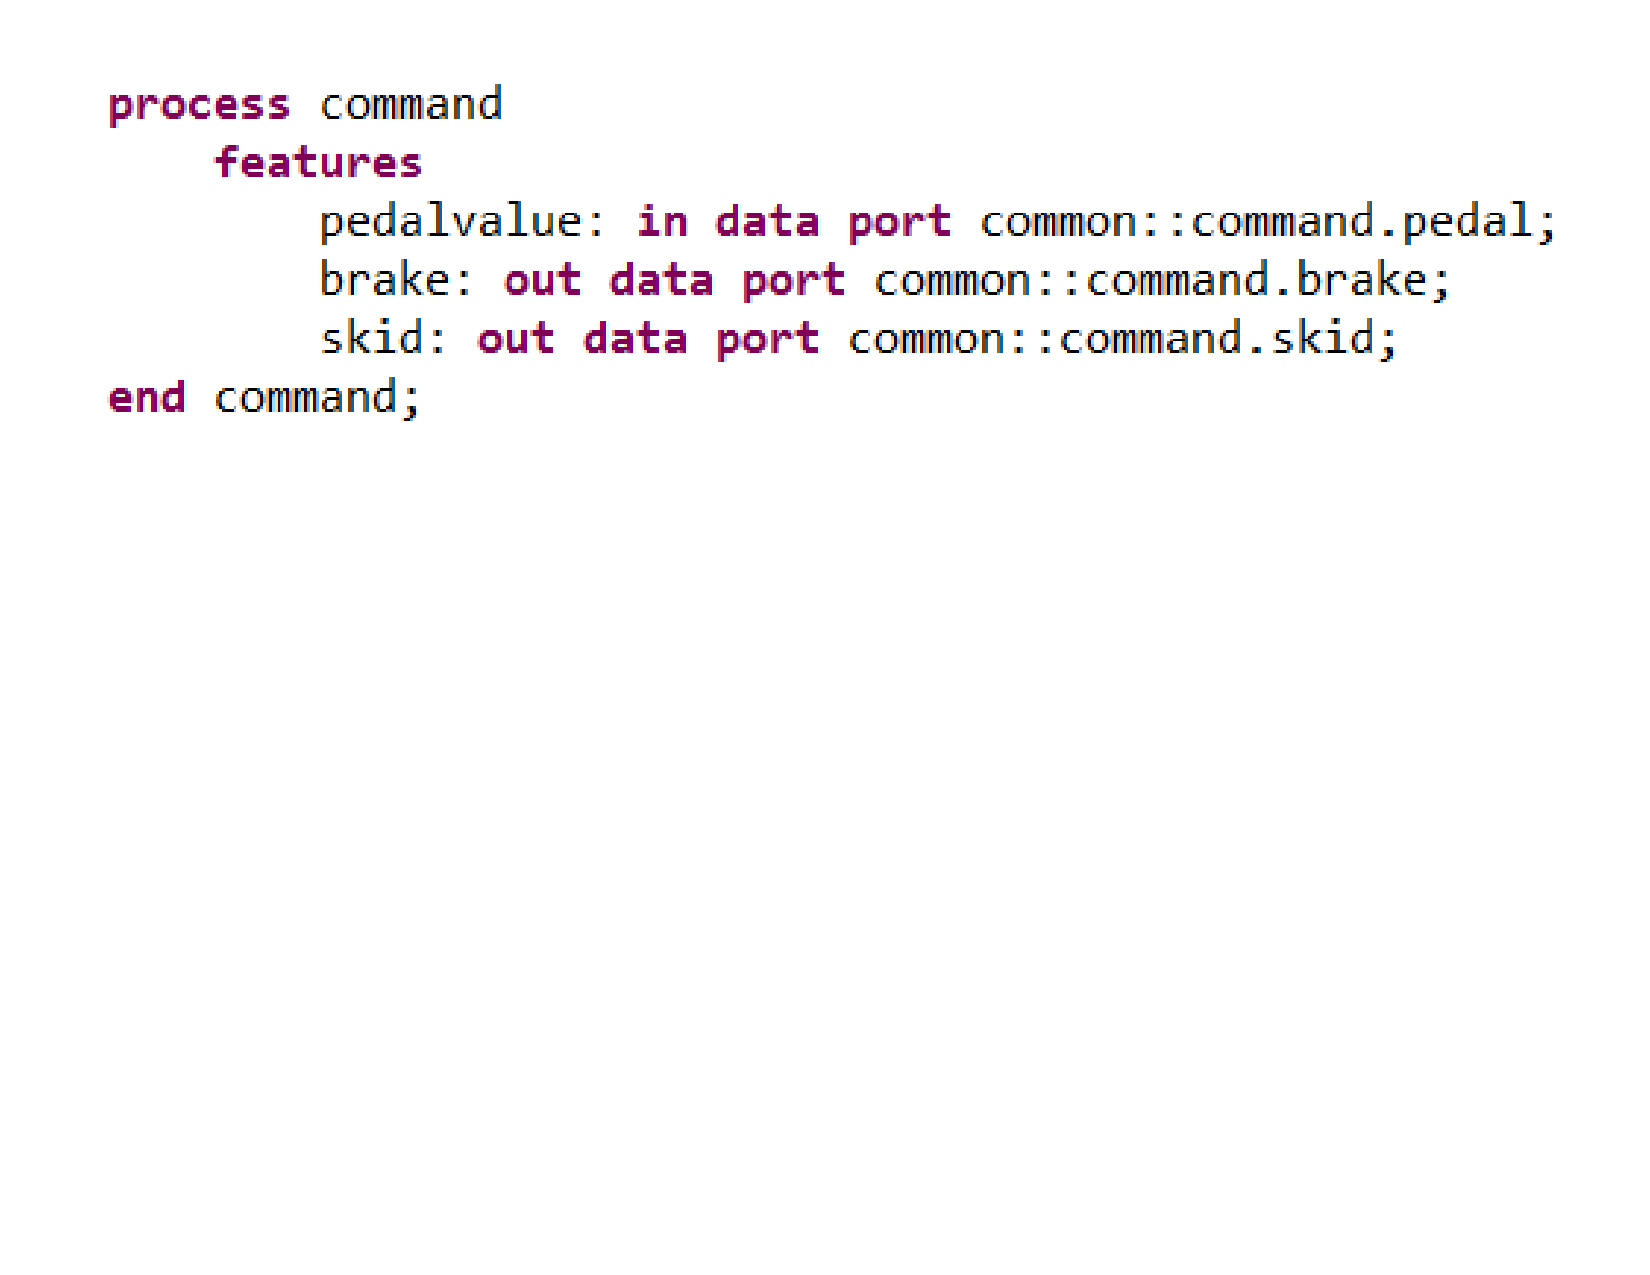
\includegraphics[clip,width=0.9\textwidth]{images/bscu_cmd_comp.pdf}
	%\vspace{-0.19in}
	\end{center}
\vspace{-2.5in}
\end{figure}

And the error propagations and component error behavior defined in EMV2 are shown below:

\begin{figure}[h!]
	\hspace*{-4cm}
	\vspace{-0.8in} 
	\begin{center}
		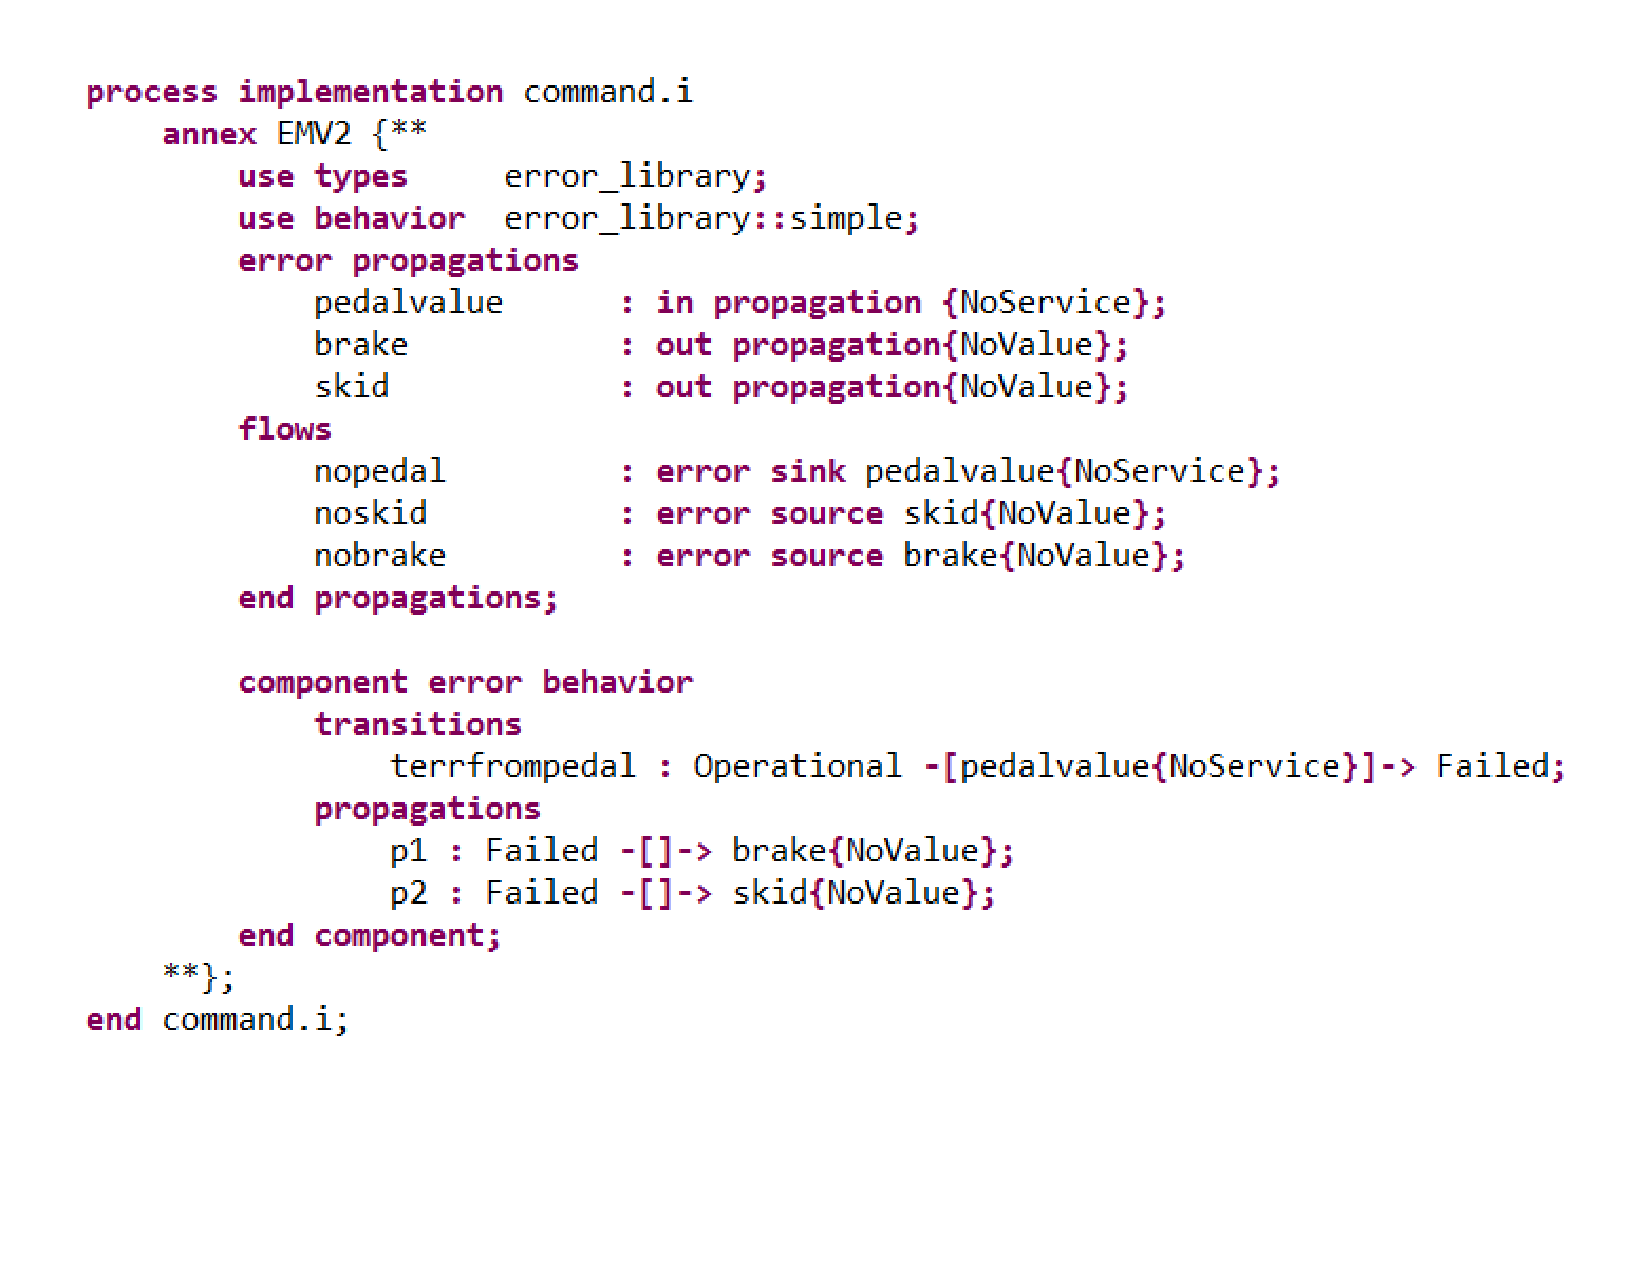
\includegraphics[width=1.5\textwidth]{images/bscu_cmd_emv2.pdf}
		%\vspace{-0.19in}
	\end{center}
	\vspace{-2.2in}
\end{figure}






 


